%%%%%%%%%%%%%%%%%%%%%%%%%%%%%%%%%%%%%%%%%
% Beamer Presentation
% LaTeX Template
% Version 1.0 (10/11/12)
%
% This template has been downloaded from:
% http://www.LaTeXTemplates.com
%
% License:
% CC BY-NC-SA 3.0 (http://creativecommons.org/licenses/by-nc-sa/3.0/)
%
%%%%%%%%%%%%%%%%%%%%%%%%%%%%%%%%%%%%%%%%%

%----------------------------------------------------------------------------------------
%	PACKAGES AND THEMES
%----------------------------------------------------------------------------------------

\documentclass[9pt]{beamer}
\usepackage{natbib}
 
\usepackage[utf8]{inputenc}
\usepackage[english]{babel}
\definecolor{maroon}{RGB}{153, 0, 0}
\usepackage[colorlinks=true, linkcolor= black, citecolor=maroon]{hyperref}
\usepackage{amsmath,amssymb,hyperref,array,xcolor,multicol,verbatim,mathpazo}



\mode<presentation> {


\usetheme{Madrid} % <<


\definecolor{UBCblue}{rgb}{0.04706, 0.13725, 0.26667} % UBC Blue
%\definecolor{lightblue}{HTML}{3498DB}  %nakamura
%\definecolor{lightblue}{HTML}{5DADE2}  %nakamura

\usecolortheme[named=UBCblue]{structure}
%\usecolortheme[named=lightblue]{structure}   %nakamura
%\setbeamercolor{button}{fg=white, bg=lightblue}  %nakamura
\usefonttheme{serif}
%\usefonttheme[onlylarge]{structuresmallcapsserif}  %nakamura

% As well as themes, the Beamer class has a number of color themes
% for any slide theme. Uncomment each of these in turn to see how it
% changes the colors of your current slide theme.

%\usecolortheme{albatross}
%\usecolortheme{beaver}
%\usecolortheme{beetle}
%\usecolortheme{crane}
%\usecolortheme{dolphin}
%\usecolortheme{dove}
%\usecolortheme{fly}
%\usecolortheme{lily}
%\usecolortheme{orchid}
%\usecolortheme{rose}
%\usecolortheme{seagull}
%\usecolortheme{seahorse}
%\usecolortheme{whale}
%\usecolortheme{wolverine}

%\setbeamertemplate{footline} % To remove the footer line in all slides uncomment this line
%\setbeamertemplate{footline}[page number] % To replace the footer line in all slides with a simple slide count uncomment this line

\setbeamertemplate{navigation symbols}{} % To remove the navigation symbols from the bottom of all slides uncomment this line
}



%----------------------------------------------------------------------------------------
%	TITLE PAGE
%----------------------------------------------------------------------------------------


\title[Measuring the Natural Rate of Interest in Brazil]{Measuring the Natural Rate of Interest in Brazil and \\
identifying its drivers: a DSGE Perspective}

\author[Alves, R.]{Renan Alves} % Your name
\institute[EESP-FGV] % Your institution as it will appear on the bottom of every slide, may be shorthand to save space
{Advisor: Prof. Dr. Marcel Ribeiro \\
Co-Advisor: Prof. Dr. Marcelo Kfoury % Your institution for the title page
%\medskip
%\textit{john@smith.com} % Your email address
}


\date{\today}

\begin{document}
\setbeamertemplate{caption}{\raggedright\insertcaption\par}
\maketitle


%%%%%%%%%%%%%%%%%%%%%%%%%%%%%%%%%%%%%%%%%%%%%%%%%%%%%%%%%%%%%%%%%
%%%%%%%%%%%%%%%%%%%%%%%%%%%%%%%%%%%%%%%%%%%%%%%%%%%%%%%%%%%%%%%%%
\begin{frame}{Introduction}
\begin{itemize}

\item When measuring the effects of monetary policy conduct on the future behavior of inflation, it is prudent to construct a measure of monetary policy stance

\item This monetary policy indicator measure is based on interest rates, it is the benchmark for the Central Bank

\item This benchmark is called the natural rate of interest

\item We refer to the natural interest rate and the natural level of the output (or potential), when prices and wages are flexible, according to \textcolor{red}{\citet{Woodford:2003}}


\end{itemize}
\end{frame}
%%%%%%%%%%%%%%%%%%%%%%%%%%%%%%%%%%%%%%%%%%%%%%%%%%%%%%%%%%%%%%%%%
%%%%%%%%%%%%%%%%%%%%%%%%%%%%%%%%%%%%%%%%%%%%%%%%%%%%%%%%%%%%%%%%%
\begin{frame}{Introduction}
\begin{itemize}


%\item For the analysis of “inflationary or deflationary pressures”, the key variable to be measured is the gap between the natural rate of interest and the interest rate controlled by the Central Bank

\item The interest rate gap, to indicate whether the monetary policy adopted was contractionary or expansionist

\item The natural interest rate is in a permanent or persistent process of decline in advanced economies \textcolor{red}{\citet{Gali:2019}}

\item Could it be that in emerging economies, such as Brazil, we also observe a reduction in the neutral interest rate?

\item What determines the neutral rate of interest in an emerging economy?

\end{itemize}
\end{frame}
%%%%%%%%%%%%%%%%%%%%%%%%%%%%%%%%%%%%%%%%%%%%%%%%%%%%%%%%%%%%%%%%%
%%%%%%%%%%%%%%%%%%%%%%%%%%%%%%%%%%%%%%%%%%%%%%%%%%%%%%%%%%%%%%%%%
\begin{frame}{Natural Interest Rate in Emerging Markets}
\begin{itemize}
    \item In emerging countries, the neutral interest rate tends not to be stable and low, unlike what happens in developed economies \textcolor{red}{\citet{Carrillo:2018}}
    
    \item In Brazil, a higher and unstable equilibrium interest rate should be expected, due to the history of high inflation and shocks of freezing of financial assets \textcolor{red}{\citet{Portugal:2009}}
    
    \item Estimates from previous work suggest that since the adoption of the inflation targeting system, the natural rate has been falling slowly over the years \textcolor{red}{\citet{Moreira:2019}}

    \item Monetary policy becomes more complicated when neutral interest is unstable as the Central Bank tries to establish the Selic rate around something moving
    
   

\end{itemize}
\end{frame}
%%%%%%%%%%%%%%%%%%%%%%%%%%%%%%%%%%%%%%%%%%%%%%%%%%%%%%%%%%%%%%%%%
%%%%%%%%%%%%%%%%%%%%%%%%%%%%%%%%%%%%%%%%%%%%%%%%%%%%%%%%%%%%%%%%%
\begin{frame}{In this paper}
\begin{itemize}
\item The aim of the paper is to estimate the natural rate of interest for the Brazilian economy and its drivers, using a New Keynesian model

\item We extended the articles of business cycles, for small open economy following \textcolor{red}{\citet{Gali:2005}} and \textcolor{red}{\citet{Lubik:2007}}, allowing preference shocks, technology shocks and external shocks.

\item The model incorporates the main characteristics of the DSGE models of small open economy and makes it possible to investigate how external shocks affect the natural rate in Brazil, during the post inflation target period

\item We evaluate the natural interest rate, using three different monetary policy rules. 
\begin{enumerate}
    \item Following the standard Taylor rule, with the central bank responding to deviation from inflation and the output gap
    
    \item The second the central bank responds to the natural interest rate and inflation (Wicksellian Rule)
    
    \item Third rule is a combination of the previous two
\end{enumerate} 


\end{itemize}
\end{frame}
%%%%%%%%%%%%%%%%%%%%%%%%%%%%%%%%%%%%%%%%%%%%%%%%%%%%%%%%%%%%%%%%%
%%%%%%%%%%%%%%%%%%%%%%%%%%%%%%%%%%%%%%%%%%%%%%%%%%%%%%%%%%%%%%%%%
\begin{frame}{Our Contribution to the Literature}
\begin{itemize}
    \item Estimate the natural rate of interest for an emerging economy, using a DSGE model
    
    \item Within the DSGE literature, the natural rate is defined as the real rate which arises in an economy in which output is at potential and inflation is at the central bank's target. We adopt this definition and compute the natural rate by shutting down nominal rigidities
    
    
    \item Use of Bayesian methods that allow to compensate the small sample with priors
    
    \item Understand how domestic and external shocks affect equilibrium interest dynamics







\end{itemize}
\end{frame}
%%%%%%%%%%%%%%%%%%%%%%%%%%%%%%%%%%%%%%%%%%%%%%%%%%%%%%%%%%%%%%%%%
%%%%%%%%%%%%%%%%%%%%%%%%%%%%%%%%%%%%%%%%%%%%%%%%%%%%%%%%%%%%%%%%%
\begin{frame}{Preliminary Results}
\begin{itemize}
    \item Natural interest rate varies over the years and has dropped consistently
    
    \item Estimates are robust for the three different monetary policy rules
    
    \item During the administration of Henrique Meirelles, the model which the central bank followed Wicksellian Rule showed the lowest average natural interest
    
    \item Under the management of Alexandre Tombini, the lowest average neutral rate was estimated with the monetary policy rule that combines the Taylor and Wicksellian rule 
    
    \item While Ilan Goldfajn was president of the central bank, the lowest neutral interest rate was found when BC followed Taylor's rule
    
\end{itemize}


\end{frame}
%%%%%%%%%%%%%%%%%%%%%%%%%%%%%%%%%%%%%%%%%%%%%%%%%%%%%%%%%%%%%%%%%
%%%%%%%%%%%%%%%%%%%%%%%%%%%%%%%%%%%%%%%%%%%%%%%%%%%%%%%%%%%%%%%%%
\begin{frame}{How do economists estimate the natural rate of interest?}
\begin{itemize}

%\item The biggest problem found in the literature is that the neutral interest rate is not observed. Because of this, several econometric techniques are used to estimate the natural interest rate

\item  The first one relies on pure time-series methods – based on
multivariate time series models: 
\begin{itemize}
    \item \textcolor{red}{Hamilton et al. (2016)}, \textcolor{red}{Del Negro et al. (2018)} and \textcolor{red}{Christensen and Rudebusch (2019)} 

\end{itemize}

\item A second approach uses semistructural econometric models:
\begin{itemize}
    \item \textcolor{red}{\citet{LW:2003}}, \textcolor{red}{\citet{HLW:2017} },\textcolor{red}{\citet{Renne:2007}}, \textcolor{red}{\citet{Wynne:2018}}, \textcolor{red}{\citet{Us:2018}}, \textcolor{red}{\citet{Lewis:2017}}
\end{itemize}

\item The third class of articles uses structural models to estimate the neutral interest rate, DSGE models:
\begin{itemize}
    \item \textcolor{red}{\citet{Neiss:2003}},
\textcolor{red}{\citet{Edge:2008}}, \textcolor{red}{\citet{Lopez-Salido:2009}}, \textcolor{red}{\citet{Bjornland:2011}}, \textcolor{red}{\citet{Justiniano:2010} }, \textcolor{red}{\citet{Melosi:2015}}, \textcolor{red}{\citet{Canzoneri:2015}}, \textcolor{red}{\citet{Curdia:2015}}, \textcolor{red}{\citet{Hristov:2016}}, \textcolor{red}{\citet{DelNegro:2017}},  \textcolor{red}{\citet{Neri:2018}}, \textcolor{red}{\citet{Grossman:2019}}, \textcolor{red}{\citet{Gali:2019}  }

\end{itemize}


\end{itemize}
\end{frame}
%%%%%%%%%%%%%%%%%%%%%%%%%%%%%%%%%%%%%%%%%%%%%%%%%%%%%%%%%%%%%%%%%
%%%%%%%%%%%%%%%%%%%%%%%%%%%%%%%%%%%%%%%%%%%%%%%%%%%%%%%%%%%%%%%%%
\begin{frame}{How do economists estimate the natural rate of interest in Brazil?}
\begin{itemize}

\item \textcolor{red}{\citet{Portugal:2009}}

\item \textcolor{red}{\citet{Moreira:2019}}

\item \textcolor{red}{\citet{Barbosa:2016}}    
\begin{itemize}
    \item Argues that the small open economy model is ideal for estimating the neutral interest rate in Brazil
    
    \item Components that affect the natural interest rate in Brazil
    \textcolor{blue}{international interest rate}; \textcolor{blue}{country risk premium}; exchange risk premium; returns on indexed bonds
\end{itemize}


\item \textcolor{red}{Neto & Candido (2018)}
\begin{itemize}
    \item Provide a simple and complementary empirical tool to evaluate the monetary policy stance in open economies that explicitly take into account the foreign output dynamic
\end{itemize}


\item \textcolor{red}{Perrelli (2019)}
\begin{itemize}
    \item Cyclic components: \textcolor{blue}{International interest rates}, \textcolor{blue}{output gap}, \textcolor{blue}{inflationary gap}, \textcolor{blue}{credit to the private sector/GDP}
    
    \item Fiscal components: BNDES loans, \textcolor{blue}{Government consumption}, Public debt/GDP, Sovereign risk
    
    \item Structural components: Demography e.g. \textcolor{red}{\citet{Ferrero:2016}}
\end{itemize}

\item \textcolor{red}{\citet{Palma:2017}}
\begin{itemize}
    \item Derive the natural rates within a New Keynesian model
    
    \item Incorporates the main ingredients of he DSGE framework
    
    \item Habit formation, Hybrid NKPC, time-varying inflation target
\end{itemize}


\end{itemize}
\end{frame}
%%%%%%%%%%%%%%%%%%%%%%%%%%%%%%%%%%%%%%%%%%%%%%%%%%%%%%%%%%%%%%%%%
%%%%%%%%%%%%%%%%%%%%%%%%%%%%%%%%%%%%%%%%%%%%%%%%%%%%%%%%%%%%%%%%%
\begin{frame}{Model’s characteristics}
\begin{itemize}
    \item Small open economy - the simplest framework \textcolor{red}{\citet{Gali:2005}} and \textcolor{red}{\citet{Lubik:2007}}
    
    \item Small size $\rightarrow$ negligible impact on the rest of the world
    \begin{itemize}
        \item Model: World economy made by a continuum of infinitesimal small economies $\Rightarrow$ SOE affected by the ROW but not affecting it; SOE as a special case of two-country model
    \end{itemize}
    
    \item Only tradable goods

    \item Household consumes imported goods and export domestically produced goods
    \begin{itemize}
        \item Monopolistic competition and sticky prices in domestic tradable goods
        
        \item Firms sets their export prices taking foreign demand as given
        
        \item Law of one price and complete exchange rate pass-through
    \end{itemize}
    
    \item Complete international financial markets
    \begin{itemize}
        \item Can perfectly insure across countries - asset for each international contingency
    \end{itemize}
    
    
    
    
\end{itemize}


\end{frame}
%%%%%%%%%%%%%%%%%%%%%%%%%%%%%%%%%%%%%%%%%%%%%%%%%%%%%%%%%%%%%%%%%
%%%%%%%%%%%%%%%%%%%%%%%%%%%%%%%%%%%%%%%%%%%%%%%%%%%%%%%%%%%%%%%%%
\begin{frame}{Model}
\begin{itemize}

\item \textcolor{red}{\citet{Grossman:2019}}, \textcolor{red}{Gali and Monacelli (2005)} and \textcolor{red}{Lubik and Schorfheide (2007)}

\item IS Curve for small open economy:

\begin{equation*}
    x_t = E_t(x_{t+1}) - \frac{1}{(1-\alpha)\tau_{\alpha}}\left(i_t - E_t(\pi_{t+1}) - r_t^{n} \right)
\end{equation*}

$\tau_{\alpha} = \frac{1}{1/\sigma + \alpha(2 - \alpha)(\eta - 1/\sigma)}$

\item The Output Gap $x_t = y_{A,t} - y_{A,t}^{n}$ and the natural interest rate $r_t^{n}$

\item The potential output of the domestic economy $y_{A,t}^{n}$ depends on the stationarized rest-of-the-world output  $y_{A,t}^{f}$ as follows: $y_{A,t}^{n} = - \Gamma_{*}y_{A,t}^{f} $

where $\Gamma_{*}=1-\sigma^{-1} \tau_{\alpha} / \sigma^{-1} \tau_{\alpha}+\sigma^{-1} \varphi$

\item The domestic output potential fluctuations that are not the result of fluctuations in domestic productivity are attributed to movements in the foreign output potential when they are out of step with those
from domestic productivity


\end{itemize}
\end{frame}
%%%%%%%%%%%%%%%%%%%%%%%%%%%%%%%%%%%%%%%%%%%%%%%%%%%%%%%%%%%%%%%%%
%%%%%%%%%%%%%%%%%%%%%%%%%%%%%%%%%%%%%%%%%%%%%%%%%%%%%%%%%%%%%%%%%
\begin{frame}{Model}
\begin{itemize}
\item The natural interest rate $r_t^{n}$ evolves according to:
\begin{equation*}
    r_t^{n} = E_t(\Delta \varepsilon_{t+1}^{c}) + \left( \frac{1 + \phi}{1 + \tau \phi} \right)E_t(z_{t+1}) + \left[\sigma -(1 - \alpha)\tau_{\alpha}(\Gamma_{*}+1)   \right]E_t(\Delta y_{A,t+1}^{f})
\end{equation*}

\item preference shock: $\varepsilon_{t+1}^{c}$ and domestic technology
growth shock $z_t = ln\left( \frac{A_t}{A_{t-1}} \right)$.

\item The New Keynesian Phillips Curve:

\begin{equation*}
    \pi_t = \beta E_t(\pi_{t+1} ) + \alpha \beta E_t(q_{t+1}) - \alpha \Delta q_t + (\tau_{\alpha} + \phi) \kappa x_t + u_t
\end{equation*}

\item The terms of trade, $q_t$. CPI inflation as follows $\pi_t = \Delta s_t + (1 - \alpha) \Delta q_t + \pi_t^{f} $

\item $\pi_t^{f}$ is world inflation which we treat as an unobservable and assume it follows an  AR(1)

\item The terms of growth rates $\Delta q_t = \tau_{\alpha}(\Delta y_{A,t}^{f} - \Delta y_{A,t})$.

\item The growth rate of the terms of trade follows an AR(1): $\Delta q_t = \rho_q \Delta q_{t-1} + \varepsilon_{q,t}$.


\end{itemize}
\end{frame}
%%%%%%%%%%%%%%%%%%%%%%%%%%%%%%%%%%%%%%%%%%%%%%%%%%%%%%%%%%%%%%%%%
%%%%%%%%%%%%%%%%%%%%%%%%%%%%%%%%%%%%%%%%%%%%%%%%%%%%%%%%%%%%%%%%%
\begin{frame}{Model}
\begin{itemize}
\item 3 differents Monetary Policy Rule.

\item A standard \textcolor{red}{Taylor (1993)}-type interest rate rule
\begin{equation*}
    i_t = \rho_i i_{t-1} + (1 - \rho_i)(\psi_{x}x_t + \psi_{\pi} \pi_t) + \varepsilon_{i,t}
\end{equation*}

\item The Wicksellian rule  (following \textcolor{red}{Cúrdia et al. (2015)}):
\begin{equation*}
    i_t = \rho_i i_{t-1} + (1 - \rho_i)(r_t^{n} + \psi_{\pi} \pi_t) + \varepsilon_{i,t}
\end{equation*}

\item With a more general rule Taylor and Wicksellian rule  (following \textcolor{red}{Cúrdia et al. (2015)}):
\begin{equation*}
    i_t = \rho_i i_{t-1} + (1 - \rho_i)(r_t^{n} + \psi_{x}x_t + \psi_{\pi} \pi_t) + \varepsilon_{i,t}
\end{equation*}


\end{itemize}
\end{frame}
%%%%%%%%%%%%%%%%%%%%%%%%%%%%%%%%%%%%%%%%%%%%%%%%%%%%%%%%%%%%%%%%%
%%%%%%%%%%%%%%%%%%%%%%%%%%%%%%%%%%%%%%%%%%%%%%%%%%%%%%%%%%%%%%%%%
\begin{frame}{Data Description}
\begin{itemize}
    \item The data used are quartely series from 2000Q1 to 2019Q4
    
    \item We use observations on real output growth, inflation, nominal interest rates, exchange rate changes, and terms of trade growth. Foreign variables: output and inflation All series are demeaned prior to estimation
    
    \begin{itemize}
        \item 	Nominal exchange rate R$/US$ - BACEN - $s_t$
        
        \item 	Terms of trade – FUNCEX - $q_t$
        
        \item 	Real domestic output – IBGE – $y_t$
        
        \item 	Domestic inflation – IBGE - $\pi_t$
        
        \item 	Nominal Interest rate: annualized Selic rate $(\%)$ – BACEN - $i_t$
        
        \item 	US inflation – FRED (Fed St. Louis) -  $\pi_t^{*}$
        
        \item US output– FRED (Fed St. Louis) -  $y_t^{*}$
    \end{itemize}
    
    
\end{itemize}
\end{frame}
%%%%%%%%%%%%%%%%%%%%%%%%%%%%%%%%%%%%%%%%%%%%%%%%%%%%%%%%%%%%%%%%%
%%%%%%%%%%%%%%%%%%%%%%%%%%%%%%%%%%%%%%%%%%%%%%%%%%%%%%%%%%%%%%%%%
\begin{frame}{Bayesian Econometric - Priors}
\begin{figure}[H]
\centering
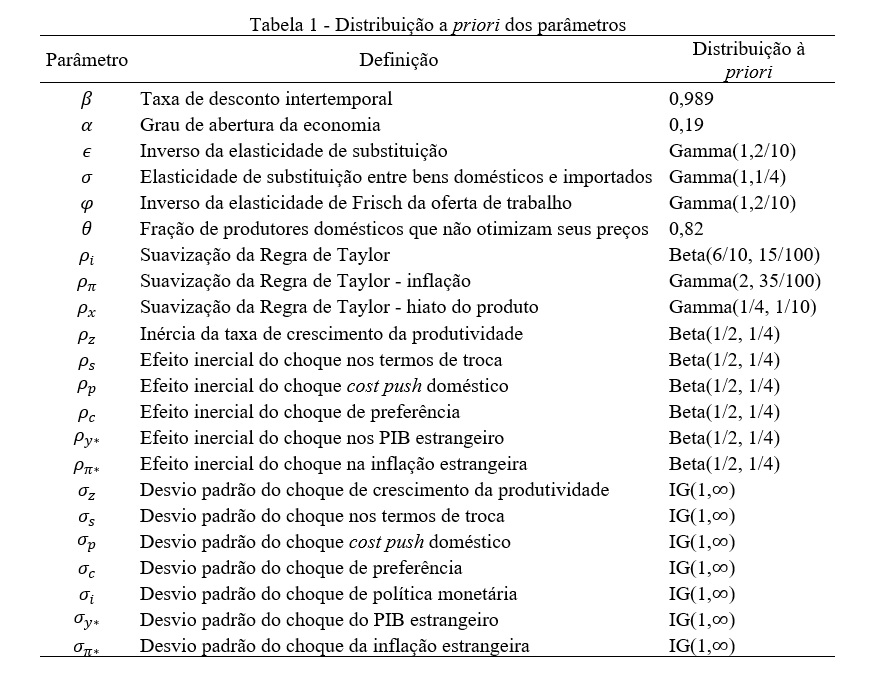
\includegraphics[scale=0.55]{Figuras/Tabelaprioris.jpg}
%\caption {\tiny Taxa Natural de Juros}
\end{figure}


\end{frame}
%%%%%%%%%%%%%%%%%%%%%%%%%%%%%%%%%%%%%%%%%%%%%%%%%%%%%%%%%%%%%%%%%
%%%%%%%%%%%%%%%%%%%%%%%%%%%%%%%%%%%%%%%%%%%%%%%%%%%%%%%%%%%%%%%%%
\begin{frame}{Results}
\begin{itemize}
    \item Taylor Rule
\end{itemize}
\begin{figure}[H]
\centering
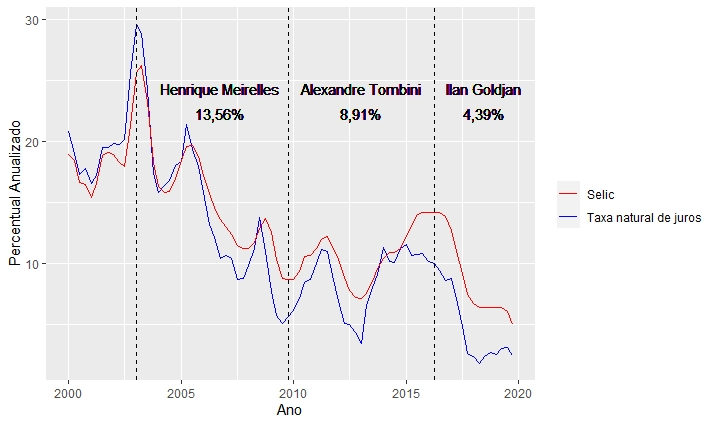
\includegraphics[scale=0.60]{Figuras/ModeloA.jpeg}
%\caption {\tiny Taxa Natural de Juros}
\end{figure}

\end{frame}
%%%%%%%%%%%%%%%%%%%%%%%%%%%%%%%%%%%%%%%%%%%%%%%%%%%%%%%%%%%%%%%%%
%%%%%%%%%%%%%%%%%%%%%%%%%%%%%%%%%%%%%%%%%%%%%%%%%%%%%%%%%%%%%%%%%
\begin{frame}{Results}
\begin{itemize}
    \item Wicksellian Rule 
\end{itemize}
\begin{figure}[H]
\centering
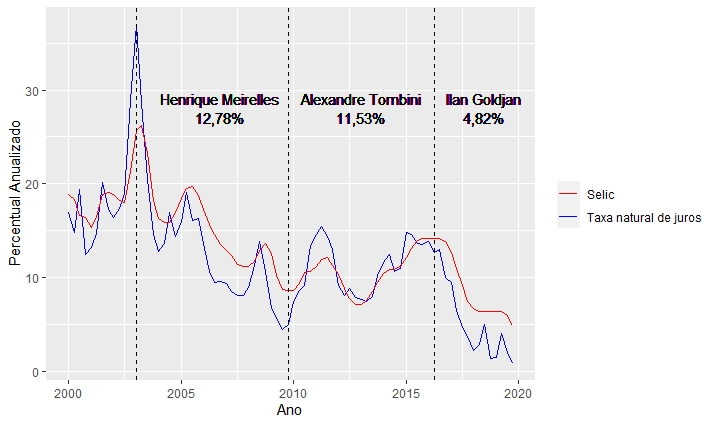
\includegraphics[scale=0.60]{Figuras/ModeloB.jpeg}
%\caption {\tiny Taxa Natural de Juros}
\end{figure}

\end{frame}
%%%%%%%%%%%%%%%%%%%%%%%%%%%%%%%%%%%%%%%%%%%%%%%%%%%%%%%%%%%%%%%%%
%%%%%%%%%%%%%%%%%%%%%%%%%%%%%%%%%%%%%%%%%%%%%%%%%%%%%%%%%%%%%%%%%
\begin{frame}{Results}
\begin{itemize}
    \item  Taylor + Wicksellian Rule
\end{itemize}
\begin{figure}[H]
\centering
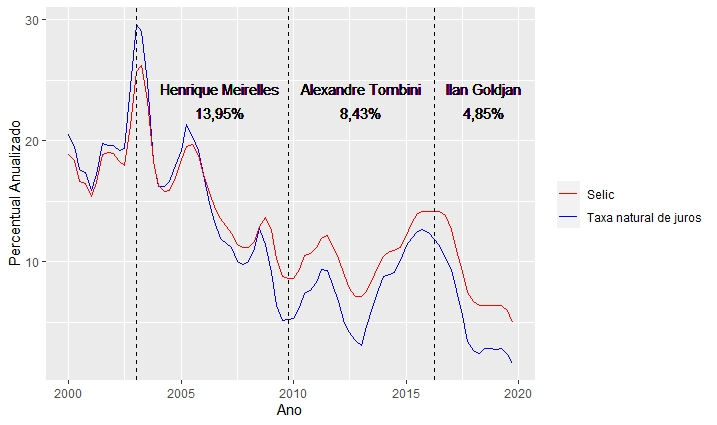
\includegraphics[scale=0.60]{Figuras/ModeloC.jpeg}
%\caption {\tiny Taxa Natural de Juros}
\end{figure}

\end{frame}
%%%%%%%%%%%%%%%%%%%%%%%%%%%%%%%%%%%%%%%%%%%%%%%%%%%%%%%%%%%%%%%%%
%%%%%%%%%%%%%%%%%%%%%%%%%%%%%%%%%%%%%%%%%%%%%%%%%%%%%%%%%%%%%%%%%
\begin{frame}{Results}
\begin{itemize}
    \item Regra Taylor + Wickseliana
\end{itemize}
\begin{figure}[H]
\centering
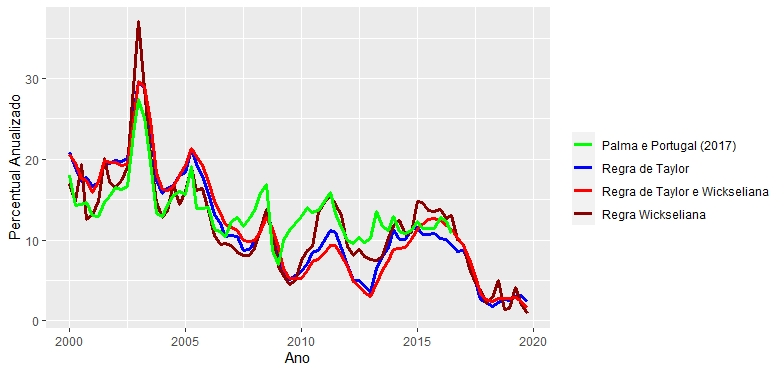
\includegraphics[scale=0.60]{Figuras/Comparativo de Juros.jpeg}
%\caption {\tiny Taxa Natural de Juros}
\end{figure}

\end{frame}
%%%%%%%%%%%%%%%%%%%%%%%%%%%%%%%%%%%%%%%%%%%%%%%%%%%%%%%%%%%%%%%%%
%%%%%%%%%%%%%%%%%%%%%%%%%%%%%%%%%%%%%%%%%%%%%%%%%%%%%%%%%%%%%%%%%
\begin{frame}{I) Next steps}

    \begin{itemize}
        \item Extend the small open economy model by following the lines of \textcolor{red}{\citet{Adolfson:2007}}, which in turn extended the models of \textcolor{red}{\citet{Christiano:2005}} and \textcolor{red}{Altig et al. (2011)} into the open economy setting
        
        \item Adding a number of variables and frictions to the standard small open economy DSGE model structure: Investment (capital accumulation), exports and imports 
        
        \item In addition, the model includes a number of additional real and nominal frictions, habit formation, such as investment adjustment costs, costly variation in the utilisation of capital and imperfect pass-through of import and export prices 
        
    
    
    
\end{itemize}


\end{frame}
%%%%%%%%%%%%%%%%%%%%%%%%%%%%%%%%%%%%%%%%%%%%%%%%%%%%%%%%%%%%%%%%%
%%%%%%%%%%%%%%%%%%%%%%%%%%%%%%%%%%%%%%%%%%%%%%%%%%%%%%%%%%%%%%%%%
\begin{frame}{II) Next steps}
    \begin{itemize}
           \item Finally, add financial frictions, along the lines of work by \textcolor{red}{Bernanke et al. (1999)}, \textcolor{red}{Christiano et al. (2014)} and \textcolor{red}{Furlanetto et at. (2020)} -  the financial accelerator mechanism distorts the economy’s response to shocks 
    
        \item We follow \textcolor{red}{\citet{Smets:2007}} the level of interest rate that emerges in the absence of dynamic distortions (sticky prices and wages) and in the absence of inefficient shocks (i.e., price mark-up and wage mark-up shocks)
        
        \item Our counterfactual is computed in the absence of both the nominal rigidities and the financial accelerator, with the aim of approximating the dynamics of the efficient frontier
        
      
    
    
\end{itemize}


\end{frame}
%%%%%%%%%%%%%%%%%%%%%%%%%%%%%%%%%%%%%%%%%%%%%%%%%%%%%%%%%%%%%%%%%
%%%%%%%%%%%%%%%%%%%%%%%%%%%%%%%%%%%%%%%%%%%%%%%%%%%%%%%%%%%%%%%%%
\begin{frame}{Model’s characteristics}
\begin{itemize}
    \item Households decide how much to consume, how much to invest and
    how much to work and at what wage
    
    \item Firms employ workers and capital and decide how much to produce
    and at what price to sell their products
    
    \item The firms (domestic, importing and exporting) all produce differentiated goods and set prices according to an indexation variant of the Calvo model
    
    \item By including nominal rigidities in the importing and exporting sectors we allow for (short-run) incomplete exchange rate pass-through to both import and export prices
    
    
    \item The central bank sets the nominal interest rate according to a Taylor rule
    
    \item There is habit formation in consumption, adjustment costs to
    investment and variable capital utilization
    
    \item The stochastic dynamics is driven by seventeen structural shocks
    
    \item  We don't model the rest of the world. We model an AR (1) process to describe world income dynamics, foreign inflation and international interest rates
    
\end{itemize}


\end{frame}
%%%%%%%%%%%%%%%%%%%%%%%%%%%%%%%%%%%%%%%%%%%%%%%%%%%%%%%%%%%%%%%%%%%%%%%%%%%%
%%%%%%%%%%%%%%%%%%%%%%%%%%%%%%%%%%%%%%%%%%%%%%%%%%%%%%%%%%%%%%%%%%%%%%%%%%%%    
\begin{frame}{Firms}
\begin{itemize}
    \item \textbf{Domestic firms} \\
    
    \textbf{Final good producers} A final good producer transforms intermediate goods into a final homogeneous good
$$
    Y_{t}=\left[\int_{0}^{1} Y_{i, t} \frac{1}{\lambda_{d, t}} d i\right]^{\lambda_{d, t}}, 1 \leq \lambda_{d, t}<\infty
$$
$\lambda_{d, t}$ is a stochastic process determining the time-varying markup in the domestic goods market
$$
\lambda_{d, t}=\left(1-\rho_{\lambda_{d}}\right) \lambda_{d}+\rho_{\lambda_{d}} \lambda_{d, t-1}+\varepsilon_{t}^{\lambda_{d}}
$$
    
Profit maximization by the final-good firm yields the demand
function for intermediate goods
$$
    Y_{i, t}=\left(\frac{P_{t}}{P_{i, t}}\right)^{\frac{\lambda_{d, t}}{\lambda_{d, t}-1}} Y_{t}
$$
    
\end{itemize}

\end{frame}
%%%%%%%%%%%%%%%%%%%%%%%%%%%%%%%%%%%%%%%%%%%%%%%%%%%%%%%%%%%%%%%%%%%%%%%%%%%%
%%%%%%%%%%%%%%%%%%%%%%%%%%%%%%%%%%%%%%%%%%%%%%%%%%%%%%%%%%%%%%%%%%%%%%%%%%%%
\begin{frame}{Intermediate good producers}
\begin{itemize}
    \item A continuum of intermediate-good producers (indexed by $i,$ where $i \in[0,1]$ ) operate in a monopolistically competitive environment and produce differentiated goods according to the production function:
$$
Y_{i, t}=\varepsilon_{t}\left(K_{i, t}\right)^{\alpha}\left(z_{t} H_{i, t}\right)^{1-\alpha}
$$
    
        
    \item $z_t$ and $\varepsilon_t$ are permanent and transitory technology shocks respectively  
  
   \item It is further assumed that the respective technology shocks follow autoregressive processes:
$$
    \begin{aligned}
    \frac{z_{t}}{z_{t-1}} &=\mu_{t}^{z} \\
    &=\left(1-\rho_{\mu^{z}}\right) \mu^{z}+\rho_{\mu^{z}} \mu_{t-1}^{z}+\epsilon_{t}^{z}
    \end{aligned}
$$
and
$$
    \hat{\varepsilon}_{t}=\rho_{\varepsilon} \hat{\varepsilon}_{t-1}+\varepsilon_{t}^{\varepsilon}
$$
where $\mu^{z}$ is the steady-state growth rate of technology, $E\left(\varepsilon_{t}\right)=1$ and $\hat{\varepsilon}_{t}=\left(\varepsilon_{t}-1\right) / 1 .$ since $\mu_{t}^{z}>1$


\end{itemize}


\end{frame}
%%%%%%%%%%%%%%%%%%%%%%%%%%%%%%%%%%%%%%%%%%%%%%%%%%%%%%%%%%%%%%%%%%%%%%%%%%%%
%%%%%%%%%%%%%%%%%%%%%%%%%%%%%%%%%%%%%%%%%%%%%%%%%%%%%%%%%%%%%%%%%%%%%%%%%%%%
\begin{frame}{Intermediate good producers}
\begin{itemize}
    \item The intermediate firm rents capital services at the gross nominal rate $R_{t}^{k}$ and compensates the homogenous labour service at the nominal wage rate $W_{t} $ 
$$
    \min _{K_{i, t}, H_{i, t}} W_{t} H_{i, t}+R_{t}^{k} K_{i, t}+\lambda_{t} P_{i, t}^{d}\left[Y_{i, t}-\varepsilon_{t}\left(K_{i, t}\right)^{\alpha}\left(z_{t} H_{i, t}\right)^{1-\alpha} \right]
$$
FOC with respect to $K_{i, t}$ and $H_{i, t}$:
$$
    R_{t}^{k}=\alpha \lambda_{t} P_{i, t} z_{t}^{1-\alpha} \epsilon_{t}\left(K_{i, t}\right)^{\alpha-1} H_{i, t}^{1-\alpha}
$$
and
$$
    W_{t}=(1-\alpha) \lambda_{t} P_{i, t} z_{t}^{1-\alpha} \epsilon_{t}\left(K_{i, t}\right)^{\alpha} H_{i, t}^{-\alpha}
$$

\item that equate the marginal returns of capital and labour to the cost of their compensation

\item where the Lagrange multiplier in Equation $\lambda_{t} P_{i, t}^{d},$ is interpreted as nominal marginal cost $M C_{t}$
    
    
    
    
\end{itemize}


\end{frame}
%%%%%%%%%%%%%%%%%%%%%%%%%%%%%%%%%%%%%%%%%%%%%%%%%%%%%%%%%%%%%%%%%%%%%%%%%%%%
%%%%%%%%%%%%%%%%%%%%%%%%%%%%%%%%%%%%%%%%%%%%%%%%%%%%%%%%%%%%%%%%%%%%%%%%%%%%
\begin{frame}{Intermediate good producers}
\begin{itemize}
    \item The stationary real rental rate of capital is expressed as:
$$
r_{t}^{k}=\frac{\alpha}{1-\alpha} \bar{w}_{t} \mu_{t}^{z}\left(\frac{H_{t}}{k_{t}}\right)
$$
and real marginal cost as
$$
m c_{t}=\left(\frac{1}{1-\alpha}\right)^{1-\alpha}\left(\frac{1}{\alpha}\right)^{\alpha} \epsilon_{t}^{-1}\left(r_{t}^{k}\right)^{\alpha}\left(\bar{w}_{t}\right)^{1-\alpha}
$$
    
%\item Because of the permanent technology shock and the unit-root in the price level, a number of variables are non-stationary as they contain a nominal and real stochastic trend. We follow \textcolor{red}{Altig et al. (2011)} and stationarize the variables in the following way
%$$
  %  r_{t}^{k} \equiv \frac{R_{t}^{k}}{P_{t}}, \bar{w}_{t} \equiv \frac{W_{t}}{P_{t} z_{t}}, k_{t+1} \equiv \frac{K_{t+1}}{z_{t}} \text { and } \bar{k}_{t+1} \equiv \frac{\bar{K}_{t+1}}{z_{t}}
%$$    
    
    
\end{itemize}


\end{frame}
%%%%%%%%%%%%%%%%%%%%%%%%%%%%%%%%%%%%%%%%%%%%%%%%%%%%%%%%%%%%%%%%%%%%%%%%%%%%
%%%%%%%%%%%%%%%%%%%%%%%%%%%%%%%%%%%%%%%%%%%%%%%%%%%%%%%%%%%%%%%%%%%%%%%%%%%%
\begin{frame}{Domestic firms setting}
\begin{itemize}
    
    
        \item It is assumed that intermediate-good firms set prices in a staggered manner as proposed by \textcolor{red}{Calvo (1983)}
        
        \item In his model a firm gets the opportunity to adjust its price with a probability of $\left( 1 - \xi_{d} \right)$ 
        
        \item With probability $\xi_{d}$ the firm is not allowed to reoptimize, and its price in period $t+1$ is then updated according to the scheme $P_{t+1}=\left(\pi_{t}\right)^{\kappa_{d}}\left(\bar{\pi}_{t+1}^{c}\right)^{1-\kappa_{d}} P_{t},$ i.e. and the current inflation target, $\bar{\pi}_{t+1}^{c}$ where $\kappa_{d}$ is an indexation parameter 
        
        \item Thus, firm $i$ faces the following optimization problem when setting its price:
        
$$\begin{aligned}
    \max _{\tilde{P}_{t}^{new}} E_{t} \sum_{s=0}^{\infty}\left(\beta \xi_{d}\right)^{s} v_{t+s}\left\{\left[\left(\prod_{k=1}^{s} \pi_{t+k-1}\right)^{\kappa_{d}}\left(\prod_{k=1}^{s} \bar{\pi}_{t+k}^{c}\right)^{1-\kappa_{d}} \tilde{P}_{t}^{new}\right]\right.& Y_{i, t+s} \\
    \left.-M C_{i, t+s}\left(Y_{i, t+s}\right)\right\} &
    \end{aligned}
$$    

  %  \item The New Keynesian Phillips curve for the domestic good:
%$$
 %   \begin{aligned}
 %   \hat{\pi}_{t}-\hat{\tilde{\pi}}_{t}^{c} &=\frac{\beta}{1+\kappa_{d} \beta}\left(E_{t} \hat{\pi}_{t+1}-\rho_{\pi} \hat{\pi}_{t}^{c}\right)+\frac{\kappa_{d}}{1+\kappa_{d} \beta}\left(\hat{\pi}_{t-1}-\hat{\tilde{\pi}}_{t}^{c}\right)-\frac{\kappa_{d} \beta\left(1-\rho_{\pi}\right)}{1+\kappa_{d} \beta} \hat{\tilde{\pi}}_{t}^{c} \\
  %  &+\frac{\left(1-\xi_{d}\right)\left(1-\beta \xi_{d}\right)}{\left(1+\kappa_{d} \beta\right) \xi_{d}}\left(\hat{m} c_{t}+\hat{\lambda}_{t}^{d}\right)
  %  \end{aligned}
%$$
    
\label{frame1}
\hyperlink{DomUnit}{\beamergotobutton{Domestic firms setting}}


\end{itemize}


\end{frame}
%%%%%%%%%%%%%%%%%%%%%%%%%%%%%%%%%%%%%%%%%%%%%%%%%%%%%%%%%%%%%%%%%%%%%%%%%%%%
%%%%%%%%%%%%%%%%%%%%%%%%%%%%%%%%%%%%%%%%%%%%%%%%%%%%%%%%%%%%%%%%%%%%%%%%%%%%
\begin{frame}{Importing Firms}
\begin{itemize}
    
        \item There are two types of importing firms:  the importing consumption  $C_{i,t}^{m}$.  While a differentiated investment good $I_{i,t}^{m}$ is created by the importing investment firm
        
        %\item Both of these importing firms purchase a homogeneous good in the world market at the international price $P_t^{*}$

        \item It is assumed that importing firms face a \textcolor{red}{Calvo (1983)} probability when setting their price. Hence, importing consumption firms may change their price with probability $\left(1 - \xi_{m,j}\right)$, for $j = \left\{ c, i\right\}$
        
        
        \item Firms who cannot reoptimise, index their price in period $t + 1$ to a combination of the previous period’s imported price inflation rate $\pi_t^{m,j}$  and the current inflation target $\bar{\pi}_{t+1}^{c}$ as follows: $P_{t+1}^{m, j}=\left(\pi_{t}^{m, j}\right)^{\kappa_{m, j}}\left(\bar{\pi}_{t+1}^{c}\right)^{1-\kappa_{m, j}} P_{t}^{m, j}$
        
        \item The consumption and investment importing firms face the following optimization problem, respectively:
        
$$\begin{array}{c}
    \max _{P_{new,t}^{m,j}} E_{t} \sum_{s=0}^{\infty}\left(\beta \xi_{m, j}\right)^{s} v_{t+s}\left\{\left[\left(\prod_{k=1}^{s} \pi_{t+k-1}^{m, j}\right)^{\kappa_{m, j}}\left(\prod_{k=1}^{s} \bar{\pi}_{t+k}^{c}\right)^{1-\kappa_{m, j}} \right. \\ \left. P_{new,t}^{m, j}\right] M_{i, t+s} -S_{t+s} P_{t+s}^{*}\left(M_{i, t+s}\right)\right\}
    \end{array}
$$
    

\end{itemize}
\label{frame2}
\hyperlink{DomUnit2}{\beamergotobutton{Importing Firms}}


\end{frame}

%%%%%%%%%%%%%%%%%%%%%%%%%%%%%%%%%%%%%%%%%%%%%%%%%%%%%%%%%%%%%%%%%%%%%%%%%%%%
%%%%%%%%%%%%%%%%%%%%%%%%%%%%%%%%%%%%%%%%%%%%%%%%%%%%%%%%%%%%%%%%%%%%%%%%%%%%
\begin{frame}{Exporting firms}
\label{frame3}
\begin{itemize}
    
    \item The demand faced by the individual exporting firm is given by:
$$
    \tilde{X}_{i, t}=\left(\frac{P_{i, t}^{x}}{P_{t}^{x}}\right)^{-\frac{\lambda_{t}^{x}}{\lambda_{t}^{x}-1}} \tilde{X}_{t}
$$    
    \item where $P_t^{x}$ is the current export price, in local currency denoted and the time-varying markup for the exporting firm is: $\lambda_{t}^{x}=\left(1-\rho_{\lambda^{x}}\right) \lambda^{x}+\rho_{\lambda^{x}} \lambda_{t-1}^{x}+\varepsilon_{t}^{\lambda^{x}}$
    
    \item To allow for incomplete exchange rate pass-through in the export market, we assume that export prices are sticky in the foreign currency follow the Calvo setup ($1 - \xi_x$)
    
    \item  The price in period t+1 is thus $P_{t+1}^{x}=\left(\pi_{t}^{x}\right)^{\kappa_{x}}\left(\bar{\pi}_{t+1}^{c}\right)^{1-\kappa_{x}} P_{t}^{x}$. The export firms maximize profits (denoted in the local currency): 
    

$$\begin{array}{c}
    \max_{P_{new,t}^{x}} E_{t} \sum_{s=0}^{\infty}\left(\beta \xi_{x, j}\right)^{s} v_{t+s}\left\{\left[\left(\prod_{k=1}^{s} \pi_{t+k-1}^{x}\right)^{\kappa_{x, j}}\left(\prod_{k=1}^{s} \bar{\pi}_{t+k}^{c}\right)^{1-\kappa_{x, j}} \right. \\ \left. P_{new,t}^{x}\right] \tilde{X}_{i,t+s}-\frac{P_{t+s}}{S_{t+s}}\left(\tilde{X}_{i, t+s}\right)\right\}
    \end{array}
$$

    
\end{itemize}

\hyperlink{DomUnit3}{\beamergotobutton{Exporting firms}}


\end{frame}
%%%%%%%%%%%%%%%%%%%%%%%%%%%%%%%%%%%%%%%%%%%%%%%%%%%%%%%%%%%%%%%%%%%%%%%%%%%%
%%%%%%%%%%%%%%%%%%%%%%%%%%%%%%%%%%%%%%%%%%%%%%%%%%%%%%%%%%%%%%%%%%%%%%%%%%%%
%\begin{frame}{Firms}
%\begin{itemize}
%    \item \textbf{Exporting firms} 
%    \begin{itemize}
 %       \item The log-linearized first order condition of this problem implies that the aggregate export inflation is given by
        
%$$\begin{aligned}
%    \left(\widehat{\pi}_{t}^{x}-\widehat{\pi}_{t}^{c}\right)=& \frac{\kappa_{x}}{1+\beta \kappa_{x}}\left(\widehat{\pi}_{t-1}^{x}-\widehat{\pi}_{t}^{c}\right)+\frac{\beta}{1+\beta \kappa_{x}}\left(\mathrm{E}_{t} \widehat{\pi}_{t+1}^{x}-\rho_{\pi} \widehat{\pi}_{t}^{c}\right) \\
%    &-\frac{\beta \kappa_{x}\left(1-\rho_{\pi}\right)}{1+\beta \kappa_{x}} \widehat{\pi}_{t}^{c}+\frac{\left(1-\beta \xi_{x}\right)\left(1-\xi_{x}\right)}{\xi_{x}\left(1+\beta \kappa_{x}\right)}\left(\widehat{m c}_{t}^{x}+\widehat{\lambda}_{x, t}\right)
%\end{aligned}$$
    
 %   \item $\widehat{mc}_t^{x} = \widehat{p}_t - \widehat{s}_t - \widehat{p}_t^{x}$
    
   % \item In the foreign economy, the exported good may either be used for consumption $C_t^{*}$ or investment $I_t^{*}$
    
   % \item foreign demand for the (aggregate) domestic consumption good, $C_t^{x}$, is given by $C_{t}^{x}=\left[\frac{P_{t}^{x}}{P_{t}^{*}}\right]^{-\eta_{f}} C_{t}^{*}$
    
%    \item foreign investment demand for the domestic good: $I_{t}^{x}=\left[\frac{P_{t}^{x}}{P_{t}^{*}}\right]^{-\eta_{f}} I_{t}^{*}$
    
%\end{itemize}
%\end{itemize}

%\end{frame}
%%%%%%%%%%%%%%%%%%%%%%%%%%%%%%%%%%%%%%%%%%%%%%%%%%%%%%%%%%%%%%%%%%%%%%%%%%%%
%%%%%%%%%%%%%%%%%%%%%%%%%%%%%%%%%%%%%%%%%%%%%%%%%%%%%%%%%%%%%%%%%%%%%%%%%%%%
\begin{frame}{The household’s problem}
\begin{itemize}
    \item Representative infinity-lived household seeking to maximize
    
    $$E_{0}^{j} \sum_{t=0}^{\infty} \beta^{t}\left[\zeta_{t}^{c} \ln \left(C_{j, t}-b C_{j, t-1}\right)-\zeta_{t}^{h} A_{L} \frac{\left(h_{j, t}\right)^{1+\sigma_{L}}}{1+\sigma_{L}}\right]$$
    
    \item  Subject to the budget constraint
$$
    \begin{aligned}
    \frac{B_{j, t}}{R_{t}} &+\frac{S_{t} B_{j, t}^{*}}{R_{t}^{*} \Phi\left(\frac{A_{t}}{z_{t}}, S_{t}, \tilde{\phi}_{t}\right)}+P_{t}^{c} C_{j, t}+P_{t}^{i} I_{j, t}+P_{t}^{d}\left[a\left(u_{j, t}\right) K_{j, t}+P_{t}^{k^{\prime}} \Delta_{t}\right] \\
    &=B_{j, t-1}+S_{t} B_{j, t-1}^{*}+W_{j, t} h_{j, t}+R_{t}^{k} u_{j, t} K_{j, t-1}+\Pi_{t}-T_{t}
    \end{aligned}
$$
    
    \item $\zeta_{t}^{c}$ and $\zeta_{t}^{h}$ represent consumption preference and labour  supply shocks, respectively. They both follow an AR(1) process:
    
    $$\begin{array}{l}
\widehat{\zeta}_{t}^{c}=\rho_{c} \widehat{\zeta}_{t-1}^{c}+\varepsilon_{t}^{\zeta_c} \\
\widehat{\zeta}_{t}^{h}=\rho_{c} \widehat{\zeta}_{t-1}^{h}+\varepsilon_{t}^{\zeta_h}
\end{array}$$    

    
    
\end{itemize}

\end{frame}


%%%%%%%%%%%%%%%%%%%%%%%%%%%%%%%%%%%%%%%%%%%%%%%%%%%%%%%%%%%%%%%%%
%%%%%%%%%%%%%%%%%%%%%%%%%%%%%%%%%%%%%%%%%%%%%%%%%%%%%%%%%%%%%%%%%
\begin{frame}{The household’s problem}
\label{frame4}
\begin{itemize}

    \item  Consumption preferences: index of domestic and imported set of goods is given by the CES index: $$C_{t}=\left[\left(1-\omega_{c}\right)^{\frac{1}{\eta_{c}}}\left(C_{t}^{d}\right)^{\frac{\eta_{c}-1}{n_{c}}}+\omega_{c}^{\frac{1}{\eta_{c}}}\left(C_{t}^{m}\right)^{\frac{\eta_{c}-1}{\eta_{c}}}\right]^{\frac{\eta_{c}}{\eta_{c}-1}}$$
    
    \item The respective demand functions for domestic and imported
    consumption goods are given by
    $$
    \begin{aligned}
    C_{t}^{d} &=\left(1-\omega_{c}\right)\left[\frac{P_{t}^{d}}{P_{t}^{c}}\right]^{-\eta_{c}} C_{t} \\
    C_{t}^{m} &=\omega_{c}\left[\frac{P_{t}^{m, c}}{P_{t}^{c}}\right]^{-\eta_{c}} C_{t}
    \end{aligned}
    $$
    
        
    \item the price index for the consumption basket (CPI) is:
    $$P_{t}^{c}=\left[\left(1-\omega_{c}\right)\left(P_{t}^{d}\right)^{1-\eta_{c}}+\omega_{c}\left(P_{t}^{m, c}\right)^{1-\eta_{c}}\right]^{\frac{1}{1-\eta_{c}}}$$
        
        
\end{itemize}

\hyperlink{DomUnit4}{\beamergotobutton{The household’s problem}}


\end{frame}
%%%%%%%%%%%%%%%%%%%%%%%%%%%%%%%%%%%%%%%%%%%%%%%%%%%%%%%%%%%%%%%%%%%%%%%%%%%%
%%%%%%%%%%%%%%%%%%%%%%%%%%%%%%%%%%%%%%%%%%%%%%%%%%%%%%%%%%%%%%%%%%%%%%%%%%%%
\begin{frame}{Investment and capital accumulation}
\begin{itemize}
    
    \item  As with consumption, households may purchase domestic ($I_t^{d}$) or imported investment goods ($I_t^{m}$), which is given by the CES aggregate:

$$I_{t}=\left[\left(1-\omega_{i}\right)^{\frac{1}{\eta_{i}}}\left(I_{t}^{d}\right)^{\frac{\eta_{i}-1}{\eta_{i}}}+\omega_{i}^{\frac{1}{\eta_{i}}}\left(I_{t}^{m}\right)^{\frac{\eta_{i}-1}{\eta_{i}}}\right]^{\frac{\eta_{i}}{\eta_{i}-1}}$$

    \item The respective demand functions for domestic and imported
    investment goods are given by
    
$$
\begin{aligned}I_{t}^{d}=\left(1-\omega_{i}\right)\left[\frac{P_{t}^{d}}{P_{t}^{i}}\right]^{-\eta_{i}} I_{t} \\ I_{t}^{m}=\omega_{i}\left[\frac{P_{t}^{m, i}}{P_{t}^{i}}\right]^{-\eta_{i}} I_{t}
\end{aligned}$$

  \item The price deflator for aggregate investment is:
    $$P_{t}^{i}=\left[\left(1-\omega_{i}\right)\left(P_{t}^{d}\right)^{1-\eta_{i}}+\omega_{i}\left(P_{t}^{m, i}\right)^{1-\eta_{i}}\right]^{\frac{1}{1-\eta_{i}}}$$
    
    
\end{itemize}

\end{frame}

%%%%%%%%%%%%%%%%%%%%%%%%%%%%%%%%%%%%%%%%%%%%%%%%%%%%%%%%%%%%%%%%%
%%%%%%%%%%%%%%%%%%%%%%%%%%%%%%%%%%%%%%%%%%%%%%%%%%%%%%%%%%%%%%%%%
\begin{frame}{Investment and capital accumulation}
\label{frame5}
\begin{itemize}
    
    \item The capital stock $K_{t+1}$ accumulates as follows:
    
     $$\bar{K}_{t}=(1-\delta) \bar{K}_{t-1}+\zeta_{t}^{i} F\left(I_{t}, I_{t-1}\right)+\Delta_{t} \text {  and  } \hat{\zeta}_{t}^{i}=\rho_{i} \hat{\zeta}_{t-1}^{i}+\varepsilon_{t}^{i} $$
    
    
    \item \textcolor{red}{\citet{Christiano:2005}} specify this adjustment cost function as follows:
    
    $$
F\left(I_{t}, I_{t-1}\right)=\left[1-S\left(\frac{I_{t}}{I_{t-1}}\right)\right] I_{t}
$$
where
$$
S\left(\frac{I_{t}}{I_{t-1}}\right)=\frac{\phi_{i}}{2}\left(\frac{I_{t}}{I_{t-1}}-\mu^{z}\right)^{2}
$$
    
    \item  in steady state S(·) satisfies $S(\mu^z) = S'(\mu^z) = 0$ and $S''(\mu^z) \equiv \phi_i $, with $\phi_i > 0$ 
    
    \item households may also choose to vary the rate at which the current capital stock is utilized, $u_t = K_t/ \bar{K}_t$
    
\end{itemize}


\hyperlink{DomUnit5}{\beamergotobutton{The household’s problem}}

\end{frame}
%%%%%%%%%%%%%%%%%%%%%%%%%%%%%%%%%%%%%%%%%%%%%%%%%%%%%%%%%%%%%%%%%%%%%%%%%%%%
%%%%%%%%%%%%%%%%%%%%%%%%%%%%%%%%%%%%%%%%%%%%%%%%%%%%%%%%%%%%%%%%%%%%%%%%%%%%
\begin{frame}{Labor supply decisions}
\begin{itemize}
    \item The differentiated labour service $h_{j,t}$ that is supplied by each household, is transformed by a labour aggregating firm into a homogeneous input good $H_t$ as follows: $$\left H_{t}=\left[\int_{0}^{1}\left(h_{j, t}\right)^{\frac{1}{\lambda_{w}}}\right]^{\lambda_{w}}$$
    
    $\lambda_w$ is the wage markup
    
    \item The demand for labour that an individual household faces is determined by $$h_{j, t}=\left[\frac{W_{j, t}}{W_{t}}\right]^{\frac{\lambda w}{1-\lambda w}} H_{t}$$
    
    \item It is assumed that a household cannot optimally set its wage in every period, but rather faces a Calvo probability $1 - \xi_w$
    
$$
    \begin{array}{c}
    W_{j, t+1}=\left(\pi_{t}^{c}\right)^{\kappa_{w}}\left(\bar{\pi}_{t+1}^{c}\right)^{\left(1-\kappa_{w}\right)} \mu_{z, t+1} W_{j, t}
    \end{array}
$$

where $ \mu_{z, t+1}=\frac{z_{t+1}}{z_{t}}$

\end{itemize}

\end{frame}
%%%%%%%%%%%%%%%%%%%%%%%%%%%%%%%%%%%%%%%%%%%%%%%%%%%%%%%%%%%%%%%%%%%%%%%%%%%%
%%%%%%%%%%%%%%%%%%%%%%%%%%%%%%%%%%%%%%%%%%%%%%%%%%%%%%%%%%%%%%%%%%%%%%%%%%%%

\begin{frame}{Labour supply and wage setting}
\begin{itemize}
    
    \item The $j^{th}$ household that can reoptimize its wage faces the following optimization problem:
    
$ 
\left\max_{W_{j, t}^{new}} E_{t} \sum_{s=0}^{\infty}\left(\beta \xi_{w}\right)^{s}\left\{\begin{array}{c}-\zeta_{t+s}^{h} A_{L} \frac{\left(h_{j, t+s}\right)^{1+\sigma_{L}}}{1+\sigma_{L}} \\ +v_{t+s} h_{j, t+s}\left[\left(\prod_{k=1}^{s} \pi_{t+k-1}^{c}\right)^{\kappa_{w}}\left(\prod_{k=1}^{s} \bar{\pi}_{t+k}^{c}\right)^{\left(1-\kappa_{w}\right)} \right. \\
\letf. \left(\prod_{k=1}^{s} \mu_{t+k}^{z}\right) W_{j, t}^{new}\right.\end{array}\right]\right\}$

    \item The first-order condition for wage setting
$E_{t} \sum_{s=0}^{\infty}\left(\beta \xi_{w}\right)^{s} h_{j, t+s}\left\{\begin{array}{c} -\zeta_{t+s}^{h} A_{L}\left(h_{j, t+s}\right)^{\sigma_{L}} \\ +\frac{\tilde{W}_{t}}{z_{t} P_{t}} \frac{z_{t+s} v_{t+s} P_{t+s}}{\lambda_{w}} \frac{\left(\frac{P_{t+s-1}^{c}}{P_{t-1}}\right)^{\kappa_{w}}\left(\prod_{k=1}^{s} \bar{\pi}_{t+k}^{c}\right)^{\left(1-\kappa_{w}\right)}}{\frac{P_{t+s}^{d}}{P_{t}^{d}}}\end{array}\right\}=0$


%    \item The wage equation:
%$
%    \hat{w}_{t}=-\frac{1}{\eta_{1}}\left[\begin{array}{l}\eta_{0} \hat{w}_{t-1}+\eta_{2} E_{t} \hat{w}_{t+1}+\eta_{3}\left(\hat{\pi}_{t}^{d}-\hat{\tilde{\pi}}_{t}^{c}\right)+\eta_{4}\left(E_{t} \hat{\pi}_{t+1}^{d}-\rho_{\pi} \hat{\tilde{\pi}}_{t}^{c}\right) \\ +\eta_{5}\left(\hat{\pi}_{t-1}^{c}-\hat{\tilde{\pi}}_{t}^{c}\right)+\eta_{6}\left(\hat{\pi}_{t}^{c}-\rho_{\pi} \hat{\tilde{\pi}}_{t}^{c}\right)+\eta_{7} \hat{\psi}_{t}^{2}+\eta_{8} \hat{H}_{t}+\eta_{9} \hat{\zeta}_{t}^{h}\end{array}\right]
%$


\end{itemize}

\end{frame}

%%%%%%%%%%%%%%%%%%%%%%%%%%%%%%%%%%%%%%%%%%%%%%%%%%%%%%%%%%%%%%%%%%%%%%%%%%%%
%%%%%%%%%%%%%%%%%%%%%%%%%%%%%%%%%%%%%%%%%%%%%%%%%%%%%%%%%%%%%%%%%%%%%%%%%%%%
\begin{frame}{Asset holdings}
\begin{itemize}

    \item  Households allocate their wealth among domestic and foreign risk-free bonds, $B_t$ and $B_t^{*}$
    
    \item The prices of these bonds are inversely proportional to their respective gross nominal interest rates, $R_t$ and $R_t^{*}$, while they have a maturity of one period
    
    \item Households purchase foreign bonds is adjusted with a risk premium that depends on the domestic economy’s indebtedness in the international asset market, as measured by its net foreign asset position:
    
    $$A_{t} \equiv \frac{S_{t} B_{t}^{*}}{P_{t}^{d}}$$
    
    \item It is assumed that the risk premium has the following functional form: $$\Phi(a_t,\tilde{\phi}_t) =
    \left(-\widetilde{\phi}_{a}\left(a_{t}-\bar{a}\right)+\tilde{\phi}_{t}\right) $$ 
    
    \item The term $\tilde{\phi}_{t}$ represents an AR(1) shock to the risk premium
    
\end{itemize}

\end{frame}
%%%%%%%%%%%%%%%%%%%%%%%%%%%%%%%%%%%%%%%%%%%%%%%%%%%%%%%%%%%%%%%%%
%%%%%%%%%%%%%%%%%%%%%%%%%%%%%%%%%%%%%%%%%%%%%%%%%%%%%%%%%%%%%%%%%
\begin{frame}{The Central Bank and Market Clearing}
\begin{itemize}
    \item \textbf{The Central Bank}
    \label{frame6}
    \begin{itemize}
     \item The monetary policy rule is specified as follows:
        $$\hat{R}_{t}=\rho_{R} \hat{R}_{t-1}+\left(1-\rho_{R}\right)\left[\hat{\bar{\pi}}_{t}^{c}+\phi_{\pi}\left(\hat{\pi}_{t+1}^{c}-\hat{\bar{\pi}}_{t}^{c}\right)+\phi_{y} \hat{y}_{t}\right]+\phi_{\Delta \pi} \hat{\pi}_{t}^{c}+\phi_{\Delta y} \Delta \hat{y}_{t}+\varepsilon_{t}^{R} $$
    \end{itemize}
    \hyperlink{DomUnit6}{\beamergotobutton{Central Bank}}
        
        \item \textbf{Market Clearing}
    
    \begin{itemize}
        \item Clearing in the domestic final goods market implies that the supply of the final-good firm should match the demand from households, government and the export market
        
        $$C_{t}^{d}+I_{t}^{d}+G_{t}+C_{t}^{x}+I_{t}^{x} \leq \varepsilon_{t}\left(K_{t}\right)^{\alpha}\left(z_{t} H_{t}\right)^{1-\alpha}-a\left(u_{t}\right) K_{t-1}$$
        
        \item Stationarising
        $$\begin{array}{l}
\quad\left(1-\omega_{c}\right)\left[\frac{P_{t}^{c}}{P_{t}^{d}}\right]^{\eta_{c}} c_{t}+\left(1-\omega_{i}\right)\left[\frac{P_{t}^{i}}{P_{t}^{d}}\right]^{\eta_{i}} i_{t}+g_{t}+\left[\frac{P_{t}^{x}}{P_{t}^{*}}\right]^{\eta_{f}} y_{t}^{*} \frac{z_{t}^{*}}{z_{t}} \\
\leq \varepsilon_{t}\left(\frac{k_{t}}{\mu_{t}^{z}}\right)^{\alpha} H_{t}^{1-\alpha}-\phi-a\left(u_{t}\right)\left(\frac{k_{t-1}}{\mu_{t}^{z}}\right)
\end{array}$$
        
    \end{itemize}
    
    
\end{itemize}

\end{frame}
%%%%%%%%%%%%%%%%%%%%%%%%%%%%%%%%%%%%%%%%%%%%%%%%%%%%%%%%%%%%%%%%%
%%%%%%%%%%%%%%%%%%%%%%%%%%%%%%%%%%%%%%%%%%%%%%%%%%%%%%%%%%%%%%%%%
%\begin{frame}{Relative prices}
%\begin{itemize}
   % \item The various price levels also need to be rendered stationary.
%    This is achieved by dividing these price levels through a numeraire. 
    
 %   \item Relative prices of consumption and investment goods:
  %  $$
  %  \gamma_{t}^{c, d} & \equiv \frac{P^{c}}{P_{t}^{d}} \text{ and }
  %  \gamma_{t}^{i, d} & \equiv \frac{P_{t}^{i}}{P_{t}^{d}}
%    $$
    
   % \item Relative prices of imported consumption and investment goods:
    
 % $$\begin{aligned}
 %   \gamma_{t}^{m c, d} & \equiv \frac{P_{t}^{m, c}}{P_{t}^{d}} \text{ and }
  %  \gamma_{t}^{m i, d} & \equiv \frac{P_{t}^{m, i}}{P_{t}^{d}}
%    \end{aligned}$$

    %\item Relative price of exported goods:
    
   % $$\gamma_{t}^{x, *} \equiv \frac{P_{t}^{x}}{P_{t}^{*}}$$
    
  %  \item  it is convenient to express both the importing and exporting firms’ marginal cost as functions of the domestic-foreign relative price
    
 %   $$\gamma_{t}^{f} \equiv \frac{P_{t}^{d}}{S_{t} P_{t}^{*}}$$
    
%\end{itemize}

%\end{frame}
%%%%%%%%%%%%%%%%%%%%%%%%%%%%%%%%%%%%%%%%%%%%%%%%%%%%%%%%%%%%%%%%%
%%%%%%%%%%%%%%%%%%%%%%%%%%%%%%%%%%%%%%%%%%%%%%%%%%%%%%%%%%%%%%%%%
%\begin{frame}{Relative prices and Foregin Inflation}%
%\begin{itemize}
%   \item \textbf{Relative prices}
 %  \begin{itemize}
%       \item the marginal cost of the importing consumption and investment good firms are given:
  %      
 %       $$\begin{array}{l}
 %       m c_{t}^{m, c} \equiv \frac{s_{t}^{T} t}{P_{t}^{m, c}}=\left(\gamma_{t}^{f} \gamma_{t}^{m c, d}\right)^{-1} \text{ and }
  %      m c_{t}^{m, i} \equiv \frac{S_{t} P_{t}^{*}}{P^{m, i}}=\left(\gamma_{t}^{f} \gamma_{t}^{m i, d}\right)^{-1} 
  %      \end{array}$$
 %       
  %      \item the exporting firm is given as:
   %     $m c_{t}^{x}=\frac{\gamma_{t}^{f}}{\gamma_{t}^{x, *}}$
        
   %\end{itemize}
   %\item \textbf{Foregin Inflation}
%    \begin{itemize}
 %       \item We don't model the rest of the world just like \textcolor{red}{\citet{Castro:2015}} does
        
  %      \item So we model an AR (1) process to describe world income dynamics, foreign inflation and international interest rates
    
   % \end{itemize} 

%\end{itemize}

%\end{frame}
%%%%%%%%%%%%%%%%%%%%%%%%%%%%%%%%%%%%%%%%%%%%%%%%%%%%%%%%%%%%%%%%%
%%%%%%%%%%%%%%%%%%%%%%%%%%%%%%%%%%%%%%%%%%%%%%%%%%%%%%%%%%%%%%%%%
% ---------------------------------------
\begin{frame}[noframenumbering]
\frametitle{Appendix}
    
Appendix
\end{frame}
%%%%%%%%%%%%%%%%%%%%%%%%%%%%%%%%%%%%%%%%%%%%%%%%%%%%%%%%%%%%%%%%%%%%%%%%%%%%%%%%%%%%%%%%%%%%%%%%%%%%%%%%%%%%%%%%%%%%%%%%%%%%%%%%%%
\begin{frame}[noframenumbering]
\frametitle{The linearised model}
\begin{itemize}
    \label{DomUnit}
    \item \textbf{Domestic Firms}
    \begin{itemize}
        \item Production
    $$
    \hat{y}_{t}=\lambda^{d}\left(\hat{\varepsilon}_{t}+\alpha\left(\hat{k}_{t}-\hat{\mu}_{t}^{z}\right)+(1-\alpha) \hat{H}_{t}\right)
    $$
    
    \item Rental rate of capital
    $$
    \hat{r}_{t}^{k}=\hat{w}_{t}+\hat{\mu}_{t}^{z}-\hat{k}_{t}+\hat{H}_{t}
    $$
    
    \item Real marginal cost
    $$
    \hat{m} c_{t}^{d}=\alpha \hat{r}_{t}^{k}+(1-\alpha)\left(\hat{w}_{t}\right)-\hat{\varepsilon}_{t}
    $$
    
    \item New Keynesian Phillips curve
    $$
    \begin{aligned}
    \hat{\pi}_{t}^{d}-\hat{\tilde{\pi}}_{t}^{c} &=\frac{\beta}{1+\beta \kappa_{d}}\left(E_{t} \hat{\pi}_{t+1}^{d}-\rho_{\pi} \hat{\bar{\pi}}_{t}^{c}\right)+\frac{\kappa_{d}}{1+\beta \kappa_{d}}\left(\hat{\pi}_{t-1}^{d}-\hat{\tilde{\pi}}_{t}^{c}\right)-\frac{\beta \kappa_{d}\left(1-\rho_{\pi}\right)}{1+\beta \kappa_{d}} \hat{\bar{\pi}}_{t}^{c} \\
    &+\frac{\left(1-\theta_{d}\right)\left(1-\beta \xi_{d}\right)}{\left(1+\beta \kappa_{d}\right) \xi_{d}}\left(\hat{m} c_{t}^{d}+\hat{\lambda}_{t}^{d}\right)
    \end{aligned}
    $$
    \end{itemize}
    
    
\end{itemize}
    
    \hyperlink{frame1}{\beamerbutton{back}}


\end{frame}
%%%%%%%%%%%%%%%%%%%%%%%%%%%%%%%%%%%%%%%%%%%%%%%%%%%%%%%%%%%%%%%%%
%%%%%%%%%%%%%%%%%%%%%%%%%%%%%%%%%%%%%%%%%%%%%%%%%%%%%%%%%%%%%%%%%
\begin{frame}[noframenumbering]
\frametitle{Importing Firms}
\begin{itemize}

    \item That each importing firm i faces the demand for imported consumption goods given by
    $$
    C_{i, t}^{m}=\left(\frac{P_{i, t}^{m, c}}{P_{t}^{m, c}}\right)^{-\frac{\lambda_{t}^{m, c}}{\lambda_{t}^{m, c}-1}} C_{t}^{m}
    $$
    
    \item the demand for the differentiated imported investment goods is given by
    $$
    I_{i, t}^{m}=\left(\frac{P_{i, t}^{m, i}}{P_{t}^{m, i}}\right)^{-\frac{\lambda_{t}^{m, i}}{\lambda_{t}^{m, i}-1}} I_{t}^{m}
    $$
    
    \item The final imported good can be expressed as a CES composite of the differentiated import goods: $M_{t}=\left[\int_{0}^{1}\left(M_{i, t}\right)^{\frac{1}{\lambda^{m, j}}} d i\right]^{\lambda_{t}^{m, j}}$
        
    \item The demand function faced by each importing firm i is given by: $M_{i, t}=\left(\frac{P_{i, t}^{m, j}}{P_{t}^{m, j}}\right)^{-\frac{\lambda_{t, j}^{m, j}}{\lambda_{t}^{m, j}-1}} M_{t}$ 
        
    \item  the time-varying markup for the imported consumption and investment goods is: $\lambda_{t}^{m, j}=\left(1-\rho_{\lambda^{m, j}}\right) \lambda^{m, j}+\rho_{\lambda^{m, j}} \lambda_{t-1}^{m, j}+\epsilon_{t}^{\lambda^{m, j}}$
        
        
    %\item Phillips curve relations for the imported consumption and investment good:
%$$\begin{aligned}
 %   \left(\widehat{\pi}_{t}^{m, j}-\widehat{\bar{\pi}}_{t}^{c}\right)=& \frac{\beta}{1+\kappa_{m, j} \beta}\left(\mathrm{E}_{t} \widehat{\pi}_{t+1}^{m, j}-\rho_{\pi} \widehat{\bar{\pi}}_{t}^{c}\right)+\frac{\kappa_{m, j}}{1+\kappa_{m, j} \beta}\left(\widehat{\pi}_{t-1}^{m, j}-\widehat{\bar{\pi}}_{t}^{c}\right) \\
  %  &-\frac{\kappa_{m, j} \beta\left(1-\rho_{\pi}\right)}{1+\kappa_{m, j} \beta} \widehat{\bar{\pi}}_{t}^{c}+\frac{\left(1-\xi_{m, j}\right)\left(1-\beta \xi_{m, j}\right)}{\xi_{m, j}\left(1+\kappa_{m, j} \beta\right)}\left(\widehat{m c}_{t}^{m, j}+\widehat{\lambda}_{t}^{m, j}\right)
%    \end{aligned}
%$$    

 %   \item $\widehat{m c}_{t}^{m, j} = \widehat{p}_t^{*} + \widehat{s}_t - \widehat{p}_t^{m,j}$ for $j = \left\{c,i \right\}$. The markup shocks, $\widehat{\lambda}_t^{m,j} $
    
    

\end{itemize}

\end{frame}
%%%%%%%%%%%%%%%%%%%%%%%%%%%%%%%%%%%%%%%%%%%%%%%%%%%%%%%%%%%%%%%%%%%%%%%%%%%%%%%%%%%%%%%%%%%%%%%%%%%%%%%%%%%%%%%%%%%%%%%%%%%%%%%%%%
\begin{frame}[noframenumbering]
\frametitle{The linearised model}
\label{DomUnit2}
\begin{itemize}
    \item \textbf{Imported goods}
    \begin{itemize}
        \item New Keynesian Phillips curve: imported consumption goods
    $$
    \begin{aligned}
    \hat{\pi}_{t}^{m, c}-\hat{\bar{\pi}}_{t}^{c} &=\frac{\beta}{1+\beta \kappa_{m, c}}\left(E_{t} \hat{\pi}_{t+1}^{m, c}-\rho_{\pi} \hat{\bar{\pi}}_{t}^{c}\right)+\frac{\kappa_{m, c}}{1+\beta \kappa_{m, c}}\left(\hat{\pi}_{t-1}^{m, c}-\hat{\bar{\pi}}_{t}^{c}\right)-\frac{\kappa_{m, c} \beta\left(1-\rho_{\pi}\right)}{1+\beta \kappa_{m, c}} \hat{\bar{\pi}}_{t}^{c} \\
    &+\frac{\left(1-\xi_{m, c}\right)\left(1-\beta \xi_{m, c}\right)}{\left(1+\beta \kappa_{m, c}\right) \xi_{m, c}}\left(\hat{m} c_{t}^{m, c}+\hat{\lambda}_{t}^{m, c}\right)
    \end{aligned}
    $$
    
    \item Marginal cost: imported consumption goods
    $$
    \hat{m} c_{t}^{m, c}=-\hat{\gamma}_{t}^{f}-\hat{\gamma}_{t}^{m c, d}
    $$

    \item New Keynesian Phillips curve: imported investment goods
    $$
    \begin{aligned}
    \hat{\pi}_{t}^{m, i}-\hat{\bar{\pi}}_{t}^{c} &=+\frac{\beta}{1+\beta \kappa_{m, i}}\left(E_{t} \hat{\pi}_{t+1}^{m, i}-\rho_{\pi} \hat{\bar{\pi}}_{t}^{c}\right)+\frac{\kappa_{m, i}}{1+\beta \kappa_{m, i}}\left(\hat{\pi}_{t-1}^{m, i}-\hat{\bar{\pi}}_{t}^{c}\right)-\frac{\kappa_{m, i} \beta\left(1-\rho_{\pi}\right)}{1+\beta \kappa_{m, i}} \hat{\bar{\pi}}_{t}^{c} \\
    &+\frac{\left(1-xi_{m, i}\right)\left(1-\beta \xi_{m, i}\right)}{\left(1+\beta x_{m, i}\right) \xi_{m, i}}\left(\hat{m} c_{t}^{m, i}+\hat{\lambda}_{t}^{m, i}\right)
    \end{aligned}
    $$

    \item Marginal cost: imported investment goods
    $$
    \hat{m} c_{t}^{m, i}=-\hat{\gamma}_{t}^{f}-\hat{\gamma}_{t}^{m i, d}
    $$

    
    \end{itemize}
    
    
\end{itemize}

    \hyperlink{frame2}{\beamerbutton{back}}


\end{frame}
%%%%%%%%%%%%%%%%%%%%%%%%%%%%%%%%%%%%%%%%%%%%%%%%%%%%%%%%%%%%%%%%%%%%%%%%%%%%%%%%%%%%%%%%%%%%%%%%%%%%%%%%%%%%%%%%%%%%%%%%%%%%%%%%%%
\begin{frame}[noframenumbering]
\frametitle{The linearised model}
\label{DomUnit3}
\begin{itemize}
    \item \textbf{Exported goods}
    \begin{itemize}
        \item 
New Keynesian Phillips curve: exported goods
$$
\begin{aligned}
\hat{\pi}_{t}^{x} - \hat{\bar{\pi}}_{t}^{c} &=\frac{\beta}{1+\beta \kappa_{x}}\left(E_{t} \hat{\pi}_{t+1}^{x}-\rho_{\pi} \hat{\pi}_{t}^{c}\right)+\frac{\kappa_{x}}{1+\beta x_{x}}\left(\hat{\pi}_{t-1}^{x}-\hat{\bar{\pi}}_{t}^{c}\right)-\frac{\kappa_{x} \beta\left(1-\rho_{\pi}\right)}{1+\beta \kappa_{x}} \hat{\bar{\pi}}_{t}^{c} \\
&+\frac{\left(1-\xi_{x}\right)\left(1-\beta \xi_{x}\right)}{\left(1+\beta \kappa_{x}\right) \xi_{x}}\left(\hat{m} c_{t}^{x}+\hat{\lambda}_{t}^{x}\right)
\end{aligned}
$$
Marginal cost: exported goods
$$
\hat{m} c_{t}^{x}=\hat{m} c_{t-1}^{x}+\hat{\pi}_{t}^{d}-\hat{\pi}_{t}^{x}-\Delta \hat{S}_{t}
$$

    
    \end{itemize}
    
    
\end{itemize}
\hyperlink{frame3}{\beamerbutton{back}}

\end{frame}
%%%%%%%%%%%%%%%%%%%%%%%%%%%%%%%%%%%%%%%%%%%%%%%%%%%%%%%%%%%%%%%%%%%%%%%%%%%%%%%%%%%%%%%%%%%%%%%%%%%%%%%%%%%%%%%%%%%%%%%%%%%%%%%%%%
\begin{frame}[noframenumbering]
\frametitle{The linearised model}
\label{DomUnit4}
\hyperlink{frame4}{\beamerbutton{back}}
\begin{itemize}
    \item \textbf{Households}
    \begin{itemize}
        \item Consumption Euler equation
        
        $$
\begin{aligned}
\hat{c}_{t} &=\frac{\mu^{2} b}{\left(\mu^{2}\right)^{2}+\beta b^{2}} \hat{c}_{t-1}+\frac{\beta \mu^{2} b}{\left(\mu^{2}\right)^{2}+\beta b^{2}} E_{t} \hat{c}_{t+1}-\frac{\mu^{2} b}{\left(\mu^{2}\right)^{2}+\beta b^{2}}\left(\hat{\mu}_{t}^{2}-\beta E_{t} \hat{\mu}_{t+1}^{2}\right) \\
&-\frac{\left(\mu^{2}-b\right)\left(\mu^{2}-\beta b\right)}{\left(\mu^{2}\right)^{2}+\beta b^{2}}\left(\hat{\psi}_{t}^{2}+\hat{\gamma}_{t}^{c, d}\right)+\frac{\mu^{2}-b}{\left(\mu^{2}\right)^{2}+\beta b^{2}}\left(\mu^{2} \hat{\xi}_{t}^{c}-\beta b E_{t} \hat{\xi}_{t+1}^{c}\right)
\end{aligned}
$$


    \item Wage setting
    
    $$
    \hat{w}_{t}=-\frac{1}{\eta_{1}}\left[\begin{array}{l}
    \eta_{0} \hat{w}_{t-1}+\eta_{2} E_{t} \hat{w}_{t+1}+\eta_{3}\left(\hat{\pi}_{t}^{d}-\hat{\tilde{\pi}}_{t}^{c}\right)+\eta_{4}\left(E_{t} \hat{\pi}_{t+1}^{d}-\rho_{\pi} \hat{\tilde{\tau}}_{t}^{c}\right) \\
    +\eta_{5}\left(\hat{\pi}_{t-1}^{c}-\hat{\tilde{\pi}}_{t}^{c}\right)+\eta_{6}\left(\hat{\pi}_{t}^{c}-\rho_{\pi} \hat{\tilde{\pi}}_{t}^{c}\right)+\eta_{7} \hat{\psi}_{t}^{2}+\eta_{8} \hat{H}_{t}+\eta_{9} \xi_{t}^{h}
    \end{array}\right]
    $$
\\
where $b_{w}=\frac{\lambda_{w} \sigma_{L}-\left(1-\lambda_{w}\right)}{\left(1-\beta \theta_{w}\right)\left(1-\theta_{w}\right)}$
$$
\left(\begin{array}{c}
\eta_{0} \\
\eta_{1} \\
\eta_{2} \\
\eta_{3} \\
\eta_{4} \\
\eta_{5} \\
\eta_{6} \\
\eta_{7} \\
\eta_{8} \\
\eta_{9}
\end{array}\right)=\left(\begin{array}{c}
b_{w} \theta_{w} \\
\lambda_{w} \sigma_{L}-b_{w}\left(1+\beta \theta_{w}^{2} \right) \\
b_{w} \beta \theta_{w} \\
-b_{w} \theta_{w} \\
b_{w} \beta \theta_{w} \\
b_{w} \theta_{w} x_{w} \\
-b_{w} \beta \theta_{w} x_{w} \\
\left(1-\lambda_{w}\right) \\
-\left(1-\lambda_{w}\right) \sigma_{L} \\
-\left(1-\lambda_{w}\right)
\end{array}\right)
$$
and $\psi_{t}^{2}$ is the stationarised Lagrange multiplier.

    
    \end{itemize}
    
    
\end{itemize}


\end{frame}
%%%%%%%%%%%%%%%%%%%%%%%%%%%%%%%%%%%%%%%%%%%%%%%%%%%%%%%%%%%%%%%%%%%%%%%%%%%%%%%%%%%%%%%%%%%%%%%%%%%%%%%%%%%%%%%%%%%%%%%%%%%%%%%%%%
\begin{frame}[noframenumbering]
\frametitle{The linearised model}
\label{DomUnit5}
\begin{itemize}
    \item \textbf{Households}
    \begin{itemize}
        \item Investment Euler equation
    $$
    \hat{i}_{t}=\frac{1}{1+\beta}\left[\beta E_{t} \hat{i}_{t+1}+\hat{i}_{t-1}+\beta E_{t} \hat{\mu}_{t+1}^{z}-\mu_{t}^{z}\right]+\frac{1}{\left(\mu^{2}\right)^{2} \phi_{i}(1+\beta)}\left(\hat{P}_{t}^{k}-\hat{\gamma}_{t}^{i, d}+\hat{\xi}_{t}^{i}\right)
    $$
    
    \item Price of installed capital
    $$
    \hat{P}_{t}^{k}=E_{t}\left[\frac{(1-\delta) \beta}{\mu^{z}} \hat{P}_{t+1}^{k}+\hat{\psi}_{t+1}^{2}-\hat{\psi}_{t}^{z}-\hat{\mu}_{t+1}^{z}+\frac{\mu^{z}-(1-\delta) \beta}{\mu^{z}} \hat{r}_{t+1}^{k}\right]
    $$
    
    \item Capital's law-of-motion
    $$
    \hat{k}_{t+1}=\frac{1-\delta}{\mu^{z}}\left(\hat{k}_{t}-\hat{\mu}_{t}^{z}\right)+\left(1-\frac{1-\delta}{\mu^{z}}\right)\left(\hat{i}_{t}+\hat{\xi}_{t}^{i}\right)
    $$
    
    \item Capital utilisation
    $$
    \hat{u}_{t}=\frac{1}{\sigma_{a}} \hat{r}_{t}^{k}
    $$
    
    \item Capital services
    $$
    \hat{k}_{t}=\hat{\bar{k}}_{t}+\hat{u}_{t}
    $$
    
   \item  Optimal asset holdings
    $$
    \hat{\psi}_{t}^{z}=E_{t}\left(\hat{\psi}_{t+1}^{z}-\hat{\mu}_{t+1}^{z}\right)+\left(\hat{R}_{t}-E_{t} \hat{\pi}_{t+1}^{d}\right)
    $$
    \item Modified UIP condition
    $$
    \hat{R}_{t}-\hat{R}_{t}^{*}=\left(1-\tilde{\phi}_{s}\right) E_{t} \Delta \hat{S}_{t+1}-\tilde{\phi}_{s} \Delta \hat{S}_{t}-\tilde{\phi}_{a} \hat{a}_{t}+\hat{\tilde{\phi}}_{t}
    $$
    
    \end{itemize}
    
    
\end{itemize}
\hyperlink{frame5}{\beamerbutton{back}}

\end{frame}
%%%%%%%%%%%%%%%%%%%%%%%%%%%%%%%%%%%%%%%%%%%%%%%%%%%%%%%%%%%%%%%%%%%%%%%%%%%%%%%%%%%%%%%%%%%%%%%%%%%%%%%%%%%%%%%%%%%%%%%%%%%%%%%%%%
\begin{frame}[noframenumbering]
\frametitle{The linearised model}
\begin{itemize}
\label{DomUnit6}


    \item \textbf{The Central Bank}
    \begin{itemize}
        \item Taylor rule
    $$
    \hat{R}_{t}=\rho_{R} \hat{R}_{t-1}+\left(1-\rho_{R}\right)\left[\hat{\tilde{\pi}}_{t}^{c}+\phi_{\pi}\left(\hat{\pi}_{t+1}^{c, 4}-\hat{\hat{\pi}}_{t}^{c}\right)+\phi_{\Delta \pi} \hat{\pi}_{t}^{c}+\phi_{y} \hat{y}_{t}+\phi_{\Delta y} \Delta \hat{y}_{t}\right]+\varepsilon_{t}^{R}
    $$
    
    \item where CPI inflation is given by
    
    $$
    \hat{\pi}_{t}^{c}=\left(1-\vartheta_{c}\right)\left(\frac{1}{\gamma^{c, d}}\right)^{1-\eta_{\epsilon}} \hat{\pi}_{t}^{d}+\vartheta_{c}\left(\gamma^{m c, c}\right)^{1-\eta_{c}} \hat{\pi}_{t}^{m, c}
    $$

    \end{itemize}
\hyperlink{frame6}{\beamerbutton{back}}

    \item \textbf{Market clearing}
    \begin{itemize}
        \item Domestic goods market
    $$
    \begin{aligned}
    \hat{y}_{t} &=\left(1-\vartheta_{c}\right)\left(\gamma^{c, d}\right)^{\eta_{c}} \frac{c}{y}\left(\hat{c}_{t}+\eta_{c} \hat{\gamma}_{t}^{c, d}\right)+\left(1-\vartheta_{i}\right)\left(\gamma^{i, d}\right)^{\eta_{i}} \frac{i}{y}\left(\hat{i}_{t}+\eta_{i} \hat{\gamma}_{t}^{i, d}\right) \\
    &+g_{y} \hat{g}_{t}+\frac{y^{*}}{y}\left(\hat{y}_{t}^{*}-\eta_{f} \hat{\gamma}_{t}^{x, *}+\hat{z}_{t}^{*}\right)+\frac{r^{k}}{\mu^{z}} \frac{k}{y}\left(\hat{k}_{t}^{s}-\hat{k}_{t}\right)
    \end{aligned}
    $$
    
    \end{itemize}
    
    \item \textbf{Foreign bond market}

    \begin{itemize}
    $$
    \begin{aligned}
    \hat{a}_{t} &=-y^{*} \hat{m} c_{t}^{x}-\eta_{f} y^{*} \hat{\gamma}_{t}^{x, *}+y^{*} \hat{y}_{t}^{*}+y^{*} \hat{z}_{t}^{*}+\left(c^{m}+i^{m}\right) \hat{\gamma}_{t}^{f} \\
    &-\left[c^{m}\left(-\eta_{c}\left(1-\vartheta_{c}\right)\left(\gamma^{c, d}\right)^{\eta_{c}-1}\right) \hat{\gamma}_{t}^{m c, d}+\hat{c}_{t}\right] \\
    &-\left[i^{m}\left(-\eta_{i}\left(1-\vartheta_{i}\right)\left(\gamma^{i, d}\right)^{\eta_{i}-1}\right) \hat{\gamma}_{t}^{m i, d}+\hat{i}_{t}\right] 
    +\frac{\pi^{*}}{\pi} \frac{1}{\beta} \hat{a}_{t-1}
    \end{aligned}
    $$
        
    \end{itemize}

    
\end{itemize}
    
\end{frame}
%%%%%%%%%%%%%%%%%%%%%%%%%%%%%%%%%%%%%%%%%%%%%%%%%%%%%%%%%%%%%%%%%%%%%%%%%%%%%%%%%%%%%%%%%%%%%%%%%%%%%%%%%%%%%%%%%%%%%%%%%%%%%%%%%%
\begin{frame}[noframenumbering]
\frametitle{The linearised model}
\begin{itemize}

\item Relative prices
    \begin{itemize}
    \item Consumption and investment goods
    $$
    \begin{aligned}
    \hat{\gamma}_{t}^{c, d} &=\hat{\gamma}_{t-1}^{i, d}+\hat{\pi}_{t}^{c}-\hat{\pi}_{t}^{d} \\
    \hat{\gamma}_{t}^{i, d} &=\hat{\gamma}_{t-1}^{i, d}+\hat{\pi}_{t}^{i}-\hat{\pi}_{t}^{d}
    \end{aligned}
    $$
    
    \item Imported consumption and investment goods
    $$
    \hat{\gamma}_{t}^{m c, d}=\hat{\gamma}_{t-1}^{m c, d}+\hat{\pi}_{t}^{m, c}-\hat{\pi}_{t}^{d}
    $$
    $$
    \hat{\gamma}_{t}^{m i, d}=\hat{\gamma}_{t-1}^{m i, d}+\hat{\pi}_{t}^{m, i}-\hat{\pi}_{t}^{d}
    $$
    
    \item Export goods
    $$
    \hat{\gamma}_{t}^{x, *}=\hat{\gamma}_{t-1}^{x, *}+\hat{\pi}_{t}^{x}-\hat{\pi}_{t}^{*}
    $$
    
    \item Domestic-foreign goods relative price
    $$
    \hat{\gamma}_{t}^{f}=\hat{m} c_{t}^{x}+\hat{\gamma}_{t}^{x, *}
    $$
    
    \item Real exchange rate
    $$
    \hat{\gamma}_{t}^{s}=-\vartheta_{c}\left(\frac{1}{\gamma^{m c, c}}\right)^{\eta_{c}-1} \hat{\gamma}_{t}^{m c, d}-\hat{\gamma}_{t}^{x, *}-\hat{m} c_{t}^{x}
    $$
    
    \end{itemize}
\end{itemize}

\end{frame}









%
%
\bibliographystyle{apalike2} %substitui o and por &
\bibliography{Bibliografia}
%
%
\end{document}
